% Please add the following required packages to your document preamble:
% \usepackage{graphicx}
\begin{table*}[]
\resizebox{\textwidth}{!}{%
\begin{tabular}{|l|l|l|l|l|l|l|l|}
\hline
\textbf{App name} & \textbf{URL}               & \textbf{\begin{tabular}[c]{@{}l@{}}Lighthouse \\ Performance \\ Score\end{tabular}} & \textbf{\begin{tabular}[c]{@{}l@{}}Average \\ Energy \\ Consumption\end{tabular}} & \textbf{\begin{tabular}[c]{@{}l@{}}L.o.c.\\ HTML\end{tabular}} & \textbf{\begin{tabular}[c]{@{}l@{}}L.o.c.\\ CSS\end{tabular}} & \textbf{\begin{tabular}[c]{@{}l@{}}L.o.c.\\ JavaScript\end{tabular}} & \textbf{\begin{tabular}[c]{@{}l@{}}Time to \\ interactive\\ (ms)\end{tabular}} \\ \hline
\rowcolor[HTML]{EFEFEF} 
awsamazoncom      & http://www.amazonaws.com   & 0.13 (Poor)                                                                                & 3078.068                                                                          & 11642                                                          & 21519                                                         & 42225                                                                & 26959.452                                                                      \\
apple             & http://www.apple.com       & 0.45 (Average)                                                                                & 175.868                                                                           & 992                                                            & 34967                                                         & 45516                                                                & 6926.777                                                                       \\
\rowcolor[HTML]{EFEFEF} 
ask               & http://www.ask.com         & 0.94 (Good)                                                                                & 39.639                                                                            & 729                                                            & 557                                                           & 11977                                                                & 3364.167                                                                       \\
china*            & http://www.china.com       & 0.08 (Poor)                                                                                & 206.624                                                                           & 2131                                                           & 3617                                                          & 19791                                                                & 14128.010                                                                      \\
\rowcolor[HTML]{EFEFEF} 
cnn               & http://www.cnn.com         & 0.01 (Poor)                                                                                & 2865.623                                                                          & 44803                                                          & 866                                                           & 153037                                                               & 32485.614                                                                      \\
coccoc            & http://www.coccoc.com      & 0.22 (Poor)                                                                                & 537.667                                                                           & 1121                                                           & 16149                                                         & 154126                                                               & 14360.126                                                                      \\
\rowcolor[HTML]{EFEFEF} 
ettoday           & http://www.ettoday.net     & 0.04 (Poor)                                                                                & 477.836                                                                           & 1599                                                           & 15989                                                         & 111295                                                               & 16075.164                                                                      \\
hao123            & http://www.hao123.com      & 0.17 (Poor)                                                                                & 323.192                                                                           & 14582                                                          & 56                                                            & 25905                                                                & 12862.119                                                                      \\
\rowcolor[HTML]{EFEFEF} 
instagram         & http://www.instagram.com   & 0.69 (Average)                                                                                & 141.857                                                                           & 12078                                                          & 0                                                             & 83393                                                                & 5609.320                                                                       \\
microsoft         & http://www.microsoft.com   & 0.86 (Good)                                                                                                                                                               & 55.150                                                                            & 3275                                                           & 94                                                            & 5548                                                                 & 3775.443                                                                       \\
\rowcolor[HTML]{EFEFEF} 
paypal            & http://www.paypal.com      & 0.63 (Average)                                                                                & 91.660                                                                            & 991                                                            & 8995                                                          & 20302                                                                & 5062.576                                                                       \\
popads            & http://www.popads.net      & 0.94 (Good)                                                                                                                                                               & 0.657                                                                             & 434                                                            & 553                                                           & 7253                                                                 & 2756.281                                                                       \\
\rowcolor[HTML]{EFEFEF} 
quora             & http://www.quora.com       & 0.59 (Average)                                                                                & 197.197                                                                           & 4377                                                           & 51492                                                         & 25800                                                                & 7745.406                                                                       \\
theguardian       & http://www.theguardian.com & 0.43 (Poor)                                                                                & 780.819                                                                           & 1337                                                           & 10785                                                         & 48699                                                                & 13140.618                                                                      \\
\rowcolor[HTML]{EFEFEF} 
tianya            & http://www.tianya.cn       & 0.52 (Average)                                                                                & 61.038                                                                            & 347                                                            & 1409                                                          & 7413                                                                 & 5156.529                                                                       \\
twitter           & http://www.twitter.com     & 0.48 (Average)                                                                                                                                                                & 191.287                                                                           & 1616                                                           & 30451                                                         & 54336                                                                & 7372.841                                                                       \\
\rowcolor[HTML]{EFEFEF} 
whatsapp          & http://www.whatsapp.com    & 0.63 (Average)                                                                                & 224.850                                                                           & 20532                                                          & 44333                                                         & 129280                                                               & 7255.729                                                                       \\
xnxx              & http://www.xnxx.com        & 0.8 (Good)                                                                                                                                                                & 124.761                                                                           & 4350                                                           & 10635                                                         & 11023                                                                & 5839.859                                                                       \\
\rowcolor[HTML]{EFEFEF} 
xvideos           & http://www.xvideos.com     & 0.76 (Good)                                                                                                                                                               & 223.455                                                                           & 5381                                                           & 25369                                                         & 23090                                                                & 6610.909                                                                       \\
yandex            & http://www.yandex.ru       & 0.83 (Good)                                                                                                                                                               & 94.201                                                                            & 20125                                                          & 5054                                                          & 62952                                                                & 5070.721                                                                       \\
\rowcolor[HTML]{EFEFEF} 
youtube           & http://www.youtube.com     & 0.75 (Good)                                                                                                                                                               & 170.904                                                                           & 25540                                                          & 12318                                                         & 163102                                                               & 6091.047                                                                       \\ \hline
\end{tabular}%
}

\caption{Web App Characteristics}
    \label{tab:design}
\end{table*}



\section{Experiment Planning}


\subsection{Context Selection}

In this particular section, we cover our context that is the environment under which we are going to perform our experiments. The context has been defined based on four dimensions proposed by Wohlin et al. \cite{Book:Exp}

The first dimension is Online versus Offline experimentation. The context of our experiment is going to be limited to mobile web apps running on the Google Chrome browser on Android device. This is an offline experiment based on the fact that the measurements are done via tools on web apps that have already been developed and published on the web, and we are not part of the development process.

The second dimension is concerned with students or professionals as subjects. Given that our concern is the energy consumption as a function of a web app's performance score, the subjects of the experiment are developers, who ultimately have a direct impact on both the score and an app's energy efficiency.

The third dimension is the nature of the experiment: toy problems vs real problems. We sampled actual web apps from the Alexa list from different performance categories, thus targeting web apps from a real world context. Furthermore, we will be conducting experiments to address a real world problem - how performance score could be an indication of energy consumption for web apps. If proven so, performance audits might help guide software developers towards developing less energy consuming web apps.

 The fourth dimension is whether our experiment is specific versus general. We are specific because we are conducting our experiment using Lighthouse as performance analyzing tool and Chrome browser on Android platform. The web apps used for the experiment are subjects from the top visited web apps with high traffic. Although we are not targeting other supported tools, browsers and platforms, we are using tools made by high regarded developers and have a good representative sample of the population. More specifically, Chrome captures over 60\% market share \cite{WEBSITE:16}. Lighthouse is developed by Google, under active development to improve its audits. Finally, Trepn was developed by Qualcomm which captures 42 percent of processors market share \cite{WEBSITE:17}. \newline


\subsection{Variable Selection}

For our research question, we consider a web app's performance score as the independent variable. We control and change our independent variables via the selection of web apps on the basis of their scores. The measurement scale for this variable is a composite score of different loading time milestones, measured in milliseconds, which are weighted, and these are compared to a benchmark of real web apps. The outcome of this process is a relative performance score placed in a log normal distribution of benchmark scores. 
The scoring range is thus between a score of one and one hundred. We concern ourselves in measuring web apps with the following fixed levels based on lighthouse score ranges \cite{WEBSITE:13}

\begin{itemize}
\item Poor: (0 - 44)
\item Average: (45 - 74)
\item Good: (75 - 100)
\newline
\end{itemize}

We consider the energy consumption as the dependent variable. We measure the consumed energy of a web app while loading it. Energy consumption is a variable calculated as the power consumed by Google Chrome to load one subject multiplied by the time the profiler has been tracking it.
\newline


\subsection{Hypothesis Formulation}
The following hypothesis were formulated to address the main research question.
To assess if the outcome of the energy consumption is related to the fixed performance levels: Poor, Average, Good - we have the following hypothesis: \newline

We test the null hypothesis that the energy consumption mean of web apps in the category low, average and high are the same: 

\[ H_0^1: \mu_{low} = \mu_{average} = \mu_{high} \]
versus the alternative that they are not the same for at least one pair: \[ H_{a}^1: \exists (i,j) | \mu_{i} != \mu_{j} \] for at least one pair (i,j). proving that they are not the same gives an idea of dependency.

\subsection{Subject Selection}
	
	The subject selection is done by a python script \cite{WEBSITE:11} which reads a csv containing the top 1 million web apps from Alexa. The script starts from the first web apps (the most visited measured by Alexa) and goes down the list until it has 100 web apps. We discard domain names where the only difference is their extension. For example if the list contains http://www.google.com and then http://www.google.ru will not be added to the list.
We use Lighthouse batch reporter to run Lighthouse tests on the list of 100 web apps, which generates 100 JSON files with Lighthouse scores \cite{WEBSITE:12}. 
We then place the web apps in categories based on their scores, these categories being poor 0-44, average 45-74, good 75-100. From each of these categories we randomly selected 7 web apps (yielding a total of 21 web apps). \newline
	
\subsection{Experiment Design}


In order to determine if there is any statistically significant
difference between the performance scores, the design will guide the statistical test needed. The statistical test is used to understand whether the energy consumption differed based on the performance score levels.

The process of selecting the right test involves considering the dependent, independent variable and proving the assumptions. 

-Energy consumption of the web app is our dependent variable which is a continuous ratio level of measurement.

-Performance score is our only independent variable with 3 treatments (Good, Average and Poor). \newline

We consider a balanced design of subjects over the different treatments, as shown in Table \ref{tab:design}. Every Treatment level contains 7 unique web apps denoted by $w_i$. Based on this design, we can consider the following tests which rely on the probability distribution of the data.


When the data meets the assumption of the outcome being sampled independently from normal populations, with possibly different population means, and with equal populations variances, we can consider one-way ANOVA. 

When the data does not meet these assumptions, Kruskal Wallis can be considered. \newline

	
\subsection{Instrumentation}

\textbf{Hardware}

For our experiment, we are using Nexus 9 tablet running on Android 5.1.1. The device is equipped with a 2.3 GHZ Dual Core processor (Denver), 2GB of RAM, a Kepler DX1 GPU and a 802.11 a/b/g/n/ac WiFi interface. Furthermore the device has a 6700 mAh Lithium-Polymer battery installed. \newline

\textbf{R and R studio}

R Studio is an IDE for R. It will be used to perform the statistical tests \cite{WEBSITE:14}. \newline

\textbf{Lighthouse}

Lighthouse is used for performance measuring. This tool simulates an Android device and loads a web app on it measuring different audits. It gives a performance score from 0 to 100 based on the specified audits.
 \newpage

\textbf{Trepn}

To measure the energy consumption we use a power and performance profiling application called 'Trepn'. This profiler estimates the energy consumed on the mobile device. To get a better indication of energy consumption of the web app, we selected the delta power consumption value in $\mu W$ which removes the drainage cause by the Android OS and the Trepn profiler itself. From Trepn we will also get the Profiling time in milliseconds. Then, Power consumption and Profiling time will be used to measure the total Energy consumption of each web apps. Web apps are run within the Google Chrome browser (version: 40.0.2214.89) with Javascript V8 3.30.33.15. \newline

\textbf{Android Runner}

For the automation of the experiment, we are using the software tool Android Task runner \cite{WEBSITE:10}. This tool will load each web app on Google Chrome and start the power profiler. After 60 seconds, the browser is closed and Trepn stops profiling. For each web app the test is performed 25 times. The energy consumption is measured for the initial load of the web app, no user interactions will be done on a web app.
\newline


\textbf{Lighthouse Batch Reporter}

This tool is used to perform a Lighthouse analysis on several web apps sequentially. We used to get the performance score of each of our selected subjects \cite{WEBSITE:12}.

\begin{figure*}
  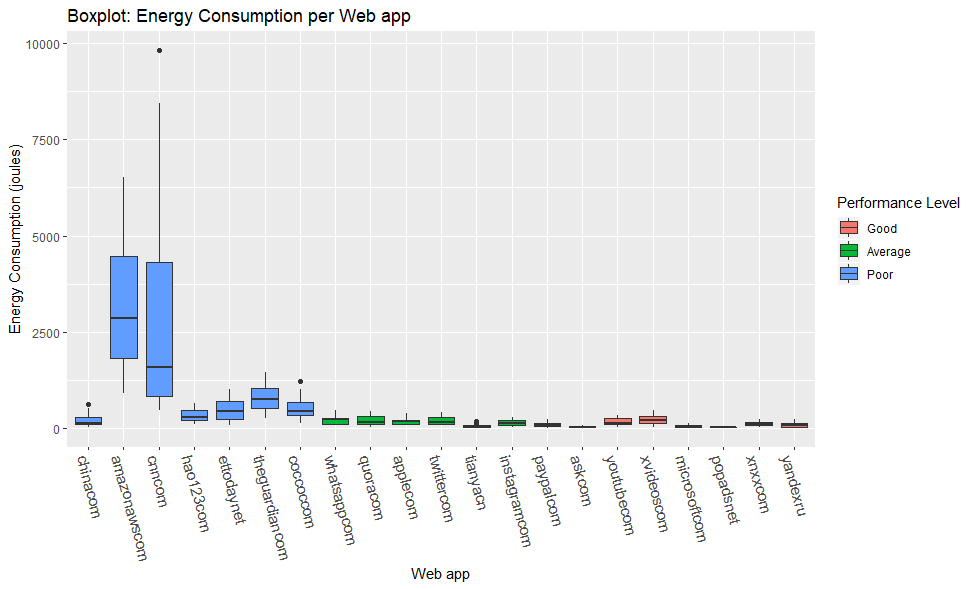
\includegraphics[width=\textwidth]{./NewImages/Fig_3_Boxplot_for_All_Websites.png}
  \caption{Boxplots for the energy consumption of all web apps}
  \label{fig:boxplots-all}
\end{figure*}